\documentclass{beamer}
% Setup appearance:
\usetheme{Marburg} 

\usepackage{color} % It may be necessary to set PCTeX or whatever program you are using to output a .pdf instead of a .dvi file in order to see color on your screen.
\usepackage{graphicx} 

\usepackage[spanish]{babel}
\usepackage[latin1]{inputenc}
\usepackage{amsmath}
\usepackage{mathtools}
\usepackage{calrsfs}
\usepackage{cases}
\usepackage{hyperref}

\usepackage{tikz}
\usetikzlibrary{arrows}
\tikzstyle{block}=[draw opacity=0.7,line width=1.4cm]


% Author, Title, etc.

\title[] 
{%
  Introducci�n al CIAA Firmware - RTOS\\ SASE 2015 %
}
	
\author[]
{
Bioing.~Juan~Manuel Reta \\ Ing. Gustavo Muro~\
}

%\insertshortdate
\date[2015]
{}


% The main document

\begin{document}

\begin{frame}
% \begin{center}

%\end{center}
  \titlepage
\begin{center}
  
	
\includegraphics[height=1cm]{Imagenes/logo_ruse}
\hspace{1cm}
	
\includegraphics[height=1cm]{Imagenes/acse}
\end{center}

\end{frame}

\section{Introducci�n}

\section{Configuraci�n}

\section{Tareas}

\subsection{Estados}

\section{Tipos de tareas}

\subsection{Prioridades}

\subsection{Scheduling}

\section{Recursos}

\subsection{Inversi�n de prioridades}

\subsection{Priotity Ceiling Protocol}

\section{Alarmas}



\section{Estructura Firmware}
\begin{frame}{Estructura Firmware}

\begin{center}
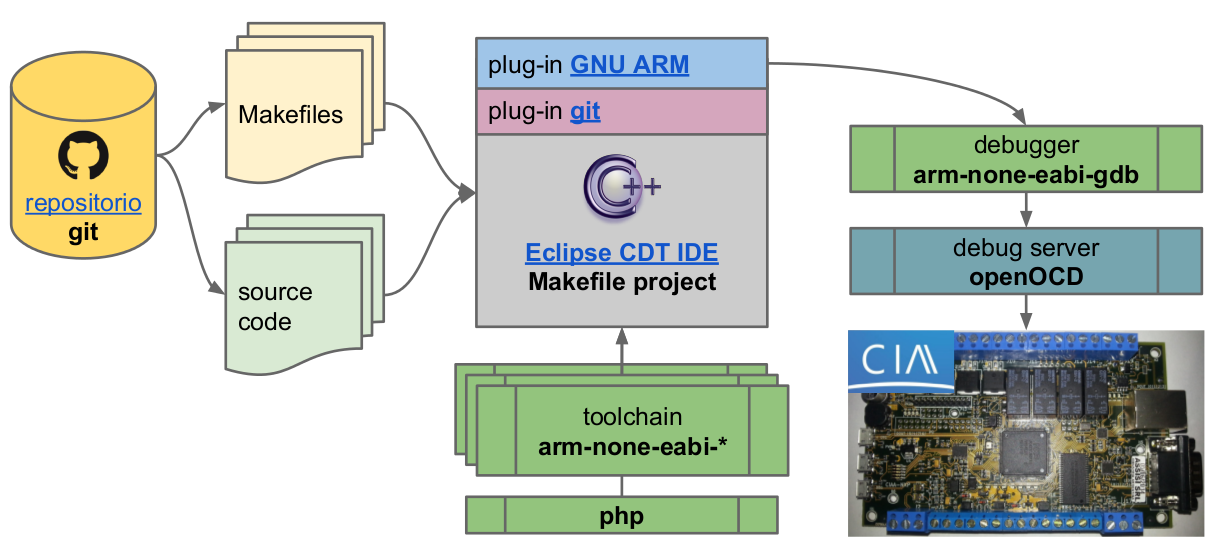
\includegraphics[height=4.5cm]{Imagenes/fimrware}
\end{center}
\begin{flushright}
{\footnotesize Fig: Ing. Pablo Ridolfi}
\end{flushright}
\end{frame}


\section{Ejercitaci�n}

\begin{frame}{}
\begin{center}

\includegraphics[height=4cm]{Imagenes/confucio}
\end{center}
\vspace{1cm}
\begin{flushright}

\includegraphics[height=2cm]{Imagenes/apredizaje}
\end{flushright}
\end{frame}


\begin{frame}{Ejercitacio 1 (Blinking)}

\begin{center}
\textbf{Explore las potencialidades de la Juntura PN}
\end{center}
\begin{center}
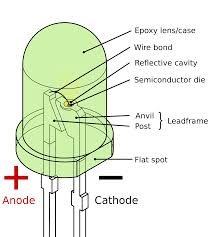
\includegraphics[height=5cm]{Imagenes/led}
\end{center}



\end{frame}
\subsection{Practica 1}

\begin{frame}{Ejercicio 2}

\begin{block}{}
Dise�e e implemente un sistema que haga parpadear un led con un
periodo de 500 ms. El sistema debe
permitir seleccionar uno de entre 4 de los leds disponibles empleando una tecla para cada led.\\

\end{block}

\begin{flushright}
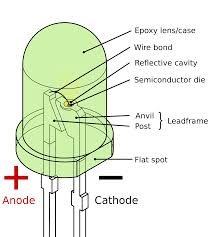
\includegraphics[height=3cm]{Imagenes/led}
\end{flushright}

\end{frame}

\begin{frame}{Ejercicio 2}

\underline{Interfaz Local:}

\begin{itemize}
\item Tec 1: Selecciona LED RGB (uno de los tres colores)
\item Tec 2: Selecciona LED 1.
\item Tec 3: Selecciona LED 2.
\item Tec 4: Selecciona LED 3.
\end{itemize}
\hspace{0.3 cm}
%\begin{columns}			
%\column{.45\textwidth}

\begin{center}
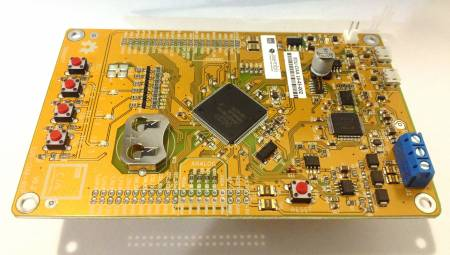
\includegraphics[height=3cm]{Imagenes/EDU_CIAA_placa}
\end{center}

%\column{.45\textwidth}
%\begin{center}

%\href{https://github.com/gmuro/ejercicioFinal}
%         {
\includegraphics[height=1cm]{Imagenes/github1}}\\
         
%Descargue la plantilla disponible en GitHub\\ (click %sobre el icono)     
%\end{center}
%\end{columns}

\end{frame}



\begin{frame}{Ejercicio 3}

\begin{block}{}
Incorpore al ejercicio anterior la funcionalidad de variar el periodo de parpadeo del led activo.\\

\end{block}

\begin{flushright}
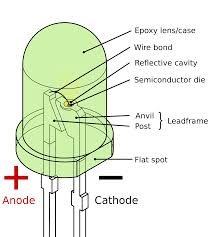
\includegraphics[height=4cm]{Imagenes/led}
\end{flushright}

\end{frame}

\begin{frame}{Ejercicio 3}

\begin{itemize}
\item Tec 1: Selecciona LED 2.
\item Tec 2: Selecciona LED 3.
\item Tec 3: Disminuye el periodo de parpadeo.
\item Tec 4: Aumenta el periodo de parpadeo.
\end{itemize}
\hspace{0.3 cm}
%\begin{columns}			
%\column{.45\textwidth}

\begin{center}
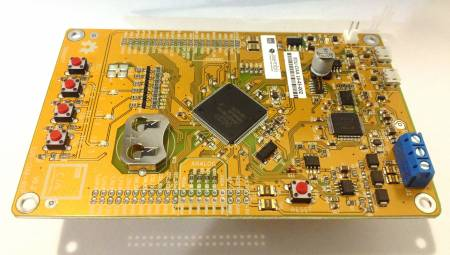
\includegraphics[height=3cm]{Imagenes/EDU_CIAA_placa}
\end{center}

%\column{.45\textwidth}
%\begin{center}

%\href{https://github.com/gmuro/ejercicioFinal}
%         {
\includegraphics[height=1cm]{Imagenes/github1}}\\
         
%Descargue la plantilla disponible en GitHub\\ (click %sobre el icono)     
%\end{center}
%\end{columns}

\end{frame}


\begin{frame}{Ejercicio 4}

\begin{block}{}

A partir de los dos ejercicios anteriores implemente un firmware que permita seleccionar uno de los 6 leds disponiblesy modificar el periodo de parpadeo \\

\end{block}

\begin{flushright}
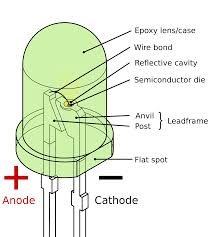
\includegraphics[height=4cm]{Imagenes/led}
\end{flushright}

\end{frame}

\begin{frame}{Ejercicio 4}

\begin{itemize}
\item Tec 1: Selecciona el led a la izquierda del actual.
\item Tec 2: Selecciona el led a la derecha del actual.
\item Tec 3: Disminuye el periodo de parpadeo.
\item Tec 4: Aumenta el periodo de parpadeo.
\end{itemize}
\hspace{0.3 cm}
%\begin{columns}			
%\column{.45\textwidth}

\begin{center}
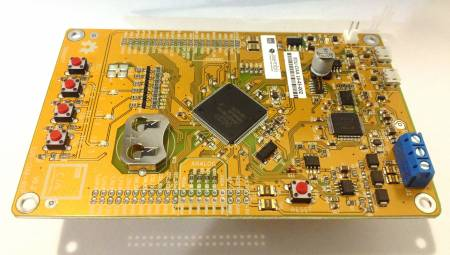
\includegraphics[height=3cm]{Imagenes/EDU_CIAA_placa}
\end{center}

%\column{.45\textwidth}
%\begin{center}

%\href{https://github.com/gmuro/ejercicioFinal}
%         {
\includegraphics[height=1cm]{Imagenes/github1}}\\
         
%Descargue la plantilla disponible en GitHub\\ (click %sobre el icono)     
%\end{center}
%\end{columns}

\end{frame}

\begin{frame}{}


\begin{center}

\includegraphics[height=4cm]{Imagenes/continuara}
\end{center}

\end{frame}

\end{document}
